% ============================================================================
% Presentaci\'on Beamer - Proyecto Final: CTF Layer 2 Security
% Redes de Computadoras - Universidad San Francisco de Quito (USFQ)
% Autores: Juli\'an Le\'on, James Soto, Mauricio Mantilla
% Fecha: Marzo 2026
% ============================================================================

\documentclass[aspectratio=169, 11pt]{beamer}

% --- Tema y colores ---
\usetheme{Madrid}
\usecolortheme{whale}
\definecolor{usfqblue}{RGB}{0, 51, 102}
\setbeamercolor{structure}{fg=usfqblue}
\setbeamercolor{title}{fg=white, bg=usfqblue}
\setbeamercolor{frametitle}{fg=white, bg=usfqblue}
\setbeamercolor{block title}{bg=usfqblue, fg=white}
\setbeamercolor{block body}{bg=usfqblue!10}
\setbeamercolor{item}{fg=usfqblue}

% --- Paquetes ---
\usepackage[utf8]{inputenc}
\usepackage[T1]{fontenc}
\usepackage[spanish]{babel}
\usepackage{graphicx}
\graphicspath{{../ctf-layer2-security/screenshots/}}
\usepackage{listings}
\usepackage{xcolor}
\usepackage{hyperref}
\usepackage{booktabs}
\usepackage{tikz}
\usetikzlibrary{shapes.geometric, arrows, positioning}

% --- Configuraci\'on de listings ---
\definecolor{codebg}{RGB}{240, 240, 240}
\definecolor{codeblue}{RGB}{30, 80, 160}
\definecolor{codegreen}{RGB}{40, 120, 40}
\definecolor{alertred}{RGB}{180, 30, 30}

\lstset{
    basicstyle=\ttfamily\scriptsize,
    backgroundcolor=\color{codebg},
    keywordstyle=\color{codeblue}\bfseries,
    stringstyle=\color{alertred},
    commentstyle=\color{codegreen}\itshape,
    frame=single,
    breaklines=true,
    showstringspaces=false,
    tabsize=2
}

% --- Metadatos ---
\title[CTF Layer 2 Security]{CTF Layer 2 Security\\[0.3em]
\large Laboratorio de Ataques y Defensas en Capa 2}
\author[Le\'on, Soto, Mantilla]{Juli\'an Le\'on \and James Soto \and Mauricio Mantilla}
\institute[USFQ]{Universidad San Francisco de Quito\\
Ingenier\'ia en Ciencias de la Computaci\'on\\[0.3em]
\textit{Redes de Computadoras}}
\date{Marzo 2026}

\begin{document}

% ============================================================================
% Slide 1: T\'itulo
% ============================================================================
\begin{frame}
\titlepage
\end{frame}

% ============================================================================
% Slide 2: Agenda
% ============================================================================
\begin{frame}{Contenido}
\tableofcontents
\end{frame}

% ============================================================================
\section{Introducci\'on}
% ============================================================================

% Slide 3: Introducci\'on y Motivaci\'on
\begin{frame}{Introducci\'on y Motivaci\'on}
\begin{block}{El problema de la Capa 2}
La mayor\'ia de mecanismos de seguridad operan en capas superiores (L3+),
dejando la Capa 2 desprotegida.
\end{block}
\vspace{0.5em}
\begin{itemize}
    \item ARP \textbf{no tiene autenticaci\'on}: cualquier host puede enviar respuestas falsas
    \item Los ataques L2 son \textbf{invisibles} para firewalls e IDS tradicionales
    \item Permiten \textbf{Man-in-the-Middle}, interceptaci\'on de tr\'afico y DoS
    \item Redes empresariales y campus universitarios son especialmente vulnerables
\end{itemize}
\vspace{0.5em}
\begin{alertblock}{Realidad}
Un atacante en la misma red local puede comprometer toda la comunicaci\'on
sin que las capas superiores lo detecten.
\end{alertblock}
\end{frame}

% ============================================================================
\section{Objetivos}
% ============================================================================

% Slide 4: Objetivos del Proyecto
\begin{frame}{Objetivos del Proyecto}
\begin{block}{Objetivo General}
Dise\~nar e implementar un laboratorio CTF que simule ataques y defensas
en Capa 2 usando tecnolog\'ias reales de ciberseguridad.
\end{block}
\vspace{0.5em}
\textbf{Objetivos Espec\'ificos:}
\begin{enumerate}
    \item Implementar ataques \textbf{ARP Spoofing} y \textbf{MAC Flooding} con Scapy
    \item Desarrollar herramientas de \textbf{detecci\'on} (Blue Team) en Python
    \item Integrar \textbf{Suricata} como NIDS con reglas personalizadas para L2
    \item Desplegar \textbf{Wazuh} como SIEM para correlaci\'on de eventos
    \item Orquestar todo en \textbf{Docker} con \textbf{CTFd} como plataforma de retos
\end{enumerate}
\end{frame}

% ============================================================================
\section{Arquitectura}
% ============================================================================

% Slide 5: Arquitectura del Laboratorio
\begin{frame}{Arquitectura del Laboratorio}
\begin{columns}[T]
\column{0.5\textwidth}
\textbf{Infraestructura:}
\begin{itemize}
    \item \textbf{13 contenedores} Docker
    \item Red bridge: \texttt{172.20.0.0/24}
    \item Orquestaci\'on con Docker Compose
\end{itemize}
\vspace{0.5em}
\textbf{Contenedores clave:}
\begin{itemize}
    \item \texttt{gateway} --- Router/gateway
    \item \texttt{victim1-3} --- Hosts v\'ictima
    \item \texttt{redteam} --- Atacante (Scapy)
    \item \texttt{blueteam} --- Defensor
    \item \texttt{suricata} --- NIDS
    \item \texttt{ctfd} --- Plataforma CTF
\end{itemize}

\column{0.5\textwidth}
\textbf{Stack Wazuh (4 contenedores):}
\begin{itemize}
    \item \texttt{wazuh.manager}
    \item \texttt{wazuh.indexer}
    \item \texttt{wazuh.dashboard}
    \item \texttt{wazuh.agent} (en blueteam)
\end{itemize}
\vspace{0.5em}
\begin{block}{Tecnolog\'ias}
\begin{itemize}
    \item Python 3 + Scapy
    \item Suricata 7.x
    \item Wazuh 4.x (SIEM/XDR)
    \item CTFd 3.x
\end{itemize}
\end{block}
\end{columns}
\end{frame}

% ============================================================================
\section{Red Team}
% ============================================================================

% Slide 6: ARP Spoofing
\begin{frame}[fragile]{Red Team --- ARP Spoofing}
\begin{columns}[T]
\column{0.55\textwidth}
\textbf{?`C\'omo funciona?}
\begin{itemize}
    \item ARP no valida respuestas $\rightarrow$ se puede falsificar
    \item El atacante env\'ia \textbf{ARP Reply} falsos a la v\'ictima
    \item La v\'ictima actualiza su tabla ARP con la MAC del atacante
    \item Resultado: tr\'afico redirigido (\textbf{MitM})
\end{itemize}
\vspace{0.5em}
\textbf{Modo broadcast:}
\begin{itemize}
    \item Env\'io a \texttt{ff:ff:ff:ff:ff:ff}
    \item Envenena \textbf{todos} los hosts simult\'aneamente
\end{itemize}

\column{0.45\textwidth}
\textbf{C\'odigo Scapy (simplificado):}
\begin{lstlisting}[language=Python]
pkt = Ether(dst="ff:ff:ff:ff:ff:ff")
    / ARP(op=2,
      psrc=gateway_ip,
      hwsrc=attacker_mac,
      pdst=victim_ip)
sendp(pkt, iface="eth0")
\end{lstlisting}
\vspace{0.3em}
\begin{alertblock}{Impacto}
Interceptaci\'on completa del tr\'afico entre v\'ictima y gateway.
\end{alertblock}
\end{columns}
\end{frame}

% Slide 7: MAC Flooding
\begin{frame}[fragile]{Red Team --- MAC Flooding}
\begin{columns}[T]
\column{0.55\textwidth}
\textbf{?`C\'omo funciona?}
\begin{itemize}
    \item Los switches tienen una \textbf{tabla CAM} de tama\~no finito
    \item Se inundan con miles de tramas con \textbf{MACs aleatorias}
    \item Al llenarse la tabla, el switch entra en modo \textbf{fail-open}
    \item El switch act\'ua como \textbf{hub}: env\'ia todo a todos los puertos
\end{itemize}
\vspace{0.5em}
\textbf{Consecuencia:}
\begin{itemize}
    \item El atacante puede capturar tr\'afico de toda la red
\end{itemize}

\column{0.45\textwidth}
\textbf{C\'odigo Scapy:}
\begin{lstlisting}[language=Python]
mac = RandMAC()
pkt = Ether(src=mac, dst=mac)
    / ARP(op=1,
      hwsrc=mac,
      psrc=RandIP())
sendp(pkt, iface="eth0",
      loop=1, inter=0.001)
\end{lstlisting}
\vspace{0.3em}
\begin{block}{Velocidad}
Miles de MACs por segundo para saturar la tabla CAM.
\end{block}
\end{columns}
\end{frame}

% ============================================================================
\section{Blue Team}
% ============================================================================

% Slide 8: Detecci\'on Blue Team
\begin{frame}{Blue Team --- Detecci\'on}
\begin{block}{ARP Monitor (H\'ibrido Activo + Pasivo)}
\begin{itemize}
    \item \textbf{Pasivo:} Captura y analiza paquetes ARP en tiempo real
    \item \textbf{Activo:} Env\'ia ARP Requests peri\'odicos para verificar consistencia
    \item Detecta cambios sospechosos en mapeos IP $\leftrightarrow$ MAC
    \item Genera alertas cuando detecta \textbf{ARP Spoofing}
\end{itemize}
\end{block}
\vspace{0.5em}
\begin{block}{MAC Anomaly Detector}
\begin{itemize}
    \item Monitorea nuevas direcciones MAC en la red
    \item Detecta \textbf{r\'afagas at\'ipicas} de MACs nuevas (umbral configurable)
    \item Identifica patrones de \textbf{MAC Flooding}
    \item Registra eventos para correlaci\'on en Wazuh
\end{itemize}
\end{block}
\end{frame}

% Slide 9: Restauraci\'on ARP
\begin{frame}{Blue Team --- Restauraci\'on ARP}
\begin{block}{Respuesta Activa}
Una vez detectado el ataque, el Blue Team puede \textbf{restaurar} las tablas ARP
de las v\'ictimas.
\end{block}
\vspace{0.5em}
\textbf{Proceso de restauraci\'on:}
\begin{enumerate}
    \item Detectar el ARP Spoofing (alerta del monitor)
    \item Obtener los mapeos \textbf{leg\'itimos} IP $\leftrightarrow$ MAC
    \item Enviar \textbf{ARP Reply correctos} a las v\'ictimas afectadas
    \item Verificar que las tablas ARP se restauraron
\end{enumerate}
\vspace{0.5em}
\begin{exampleblock}{Resultado}
Las v\'ictimas recuperan los mapeos ARP leg\'itimos y el tr\'afico
vuelve a fluir por la ruta correcta.
\end{exampleblock}
\end{frame}

% ============================================================================
\section{Suricata NIDS}
% ============================================================================

% Slide 10: Suricata
\begin{frame}[fragile]{Suricata --- Sistema de Detecci\'on de Intrusos}
\begin{block}{Desaf\'io}
Suricata no soporta \texttt{arp} como protocolo directamente en reglas.
Se usa \textbf{pkthdr} para inspeccionar tramas a nivel de enlace.
\end{block}
\vspace{0.5em}
\textbf{7 reglas personalizadas} para detecci\'on L2:
\begin{itemize}
    \item Detecci\'on de \textbf{ARP Reply} sospechosos (alto volumen)
    \item Detecci\'on de \textbf{ARP broadcast} an\'omalos
    \item Identificaci\'on de patrones de \textbf{MAC Flooding}
    \item Alertas por cambios r\'apidos en mapeos ARP
\end{itemize}
\vspace{0.5em}
\textbf{Ejemplo de regla:}
\begin{lstlisting}
alert pkthdr any any -> any any (msg:"ARP
  Spoofing detectado"; content:"|00 06|";
  offset:12; depth:2; sid:1000001; rev:1;)
\end{lstlisting}
\end{frame}

% ============================================================================
\section{Wazuh SIEM}
% ============================================================================

% Slide 11: Wazuh SIEM
\begin{frame}{Wazuh --- SIEM y Correlaci\'on de Eventos}
\begin{columns}[T]
\column{0.5\textwidth}
\textbf{Integraci\'on:}
\begin{itemize}
    \item Logs compartidos v\'ia \textbf{vol\'umenes Docker}
    \item Suricata $\rightarrow$ \texttt{eve.json} $\rightarrow$ Wazuh
    \item Blue Team scripts $\rightarrow$ logs $\rightarrow$ Wazuh
\end{itemize}
\vspace{0.5em}
\textbf{Reglas personalizadas:}
\begin{itemize}
    \item IDs: \texttt{100010} -- \texttt{100021}
    \item Niveles de severidad 5--12
    \item Correlaci\'on de m\'ultiples fuentes
\end{itemize}

\column{0.5\textwidth}
\textbf{Capacidades:}
\begin{itemize}
    \item Dashboard centralizado
    \item Threat Hunting interactivo
    \item Visualizaci\'on de alertas L2
    \item Historial de eventos
\end{itemize}
\vspace{0.5em}
\begin{block}{Ventaja}
Visibilidad completa de ataques L2 desde una \textbf{\'unica consola},
correlacionando datos de Suricata y scripts Blue Team.
\end{block}
\end{columns}
\end{frame}

% ============================================================================
\section{Demo y Resultados}
% ============================================================================

% Slide 12: Resultados del CTF
\begin{frame}{Demo --- Resultados del CTF}
\begin{block}{Retos completados: 3/3 flags capturados}
\end{block}
\vspace{0.5em}
\begin{table}[h]
\centering
\begin{tabular}{lll}
\toprule
\textbf{Reto} & \textbf{Flag} & \textbf{Puntos} \\
\midrule
ARP Spoofing & \texttt{FLAG\{arp\_spoof\_detected\}} & 100 \\
MAC Flooding & \texttt{FLAG\{mac\_flood\_detected\}} & 100 \\
Restauraci\'on & \texttt{FLAG\{arp\_restored\}} & 150 \\
\bottomrule
\end{tabular}
\end{table}
\vspace{0.5em}
\textbf{Flujo del CTF:}
\begin{enumerate}
    \item Red Team ejecuta el ataque
    \item Blue Team detecta y genera evidencia
    \item Se valida la flag en \textbf{CTFd}
    \item SIEM registra todo el proceso
\end{enumerate}
\end{frame}

% ============================================================================
\section{Evidencia}
% ============================================================================

% Slide 13: Wazuh Overview
\begin{frame}{Evidencia --- Wazuh Dashboard Overview}
\begin{center}
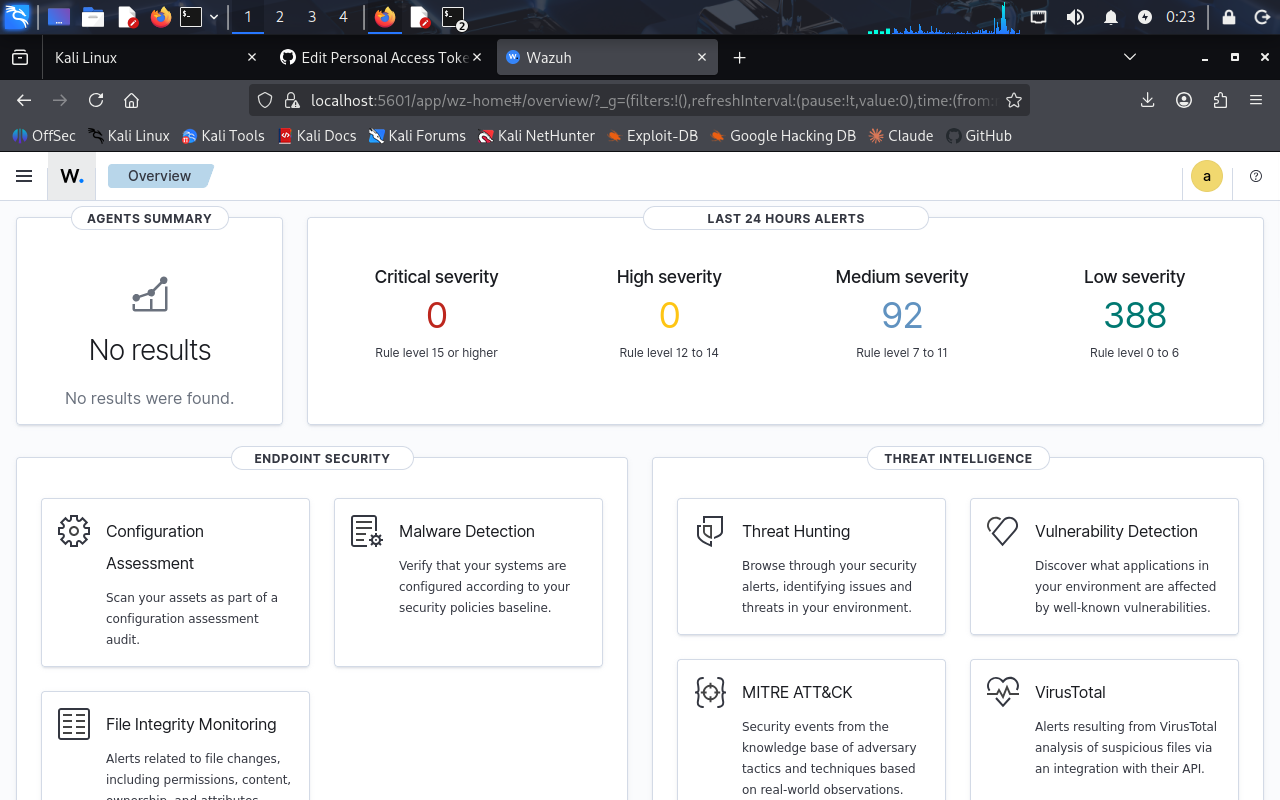
\includegraphics[width=0.85\textwidth]{woverview.png}
\end{center}
\vspace{-0.5em}
\begin{center}
\small Vista general del dashboard de Wazuh mostrando alertas de seguridad L2.
\end{center}
\end{frame}

% Slide 14: Wazuh Threat Hunting
\begin{frame}{Evidencia --- Wazuh Threat Hunting}
\begin{center}
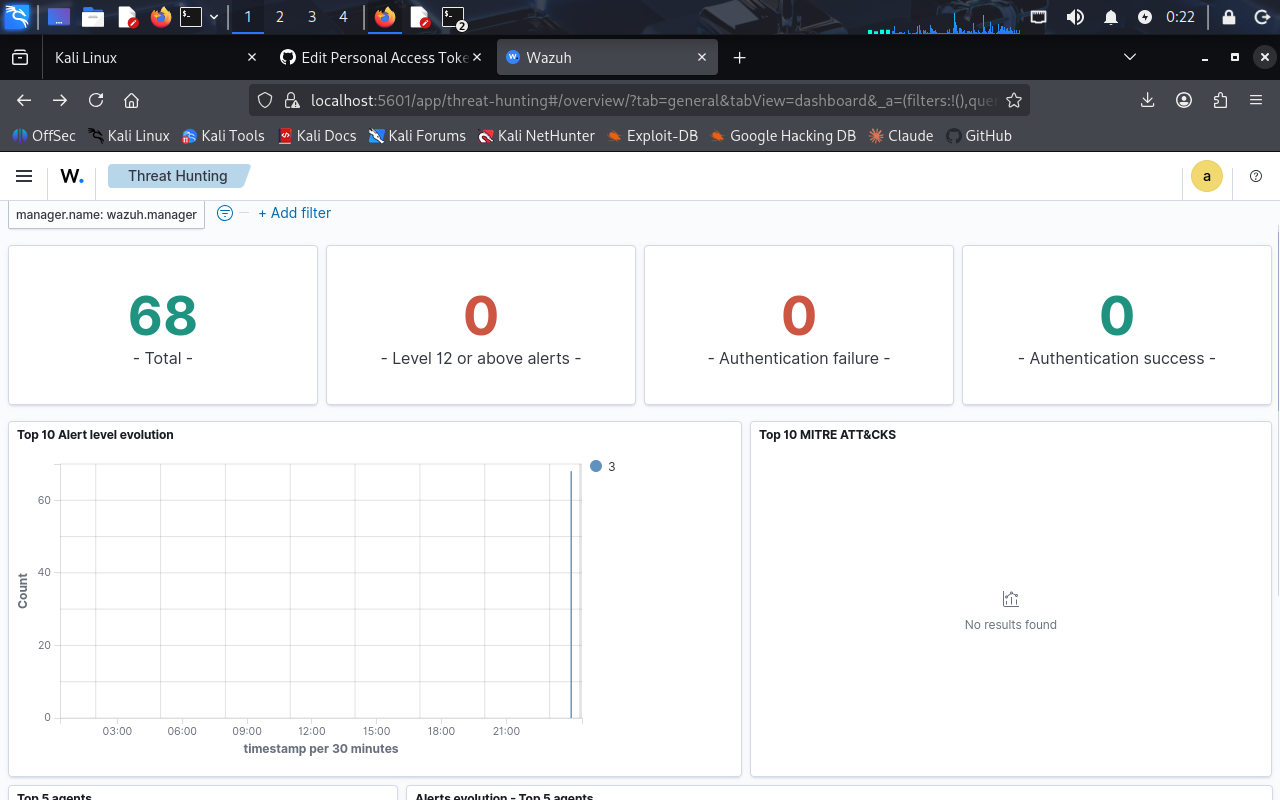
\includegraphics[width=0.85\textwidth]{wthreathunting.png}
\end{center}
\vspace{-0.5em}
\begin{center}
\small M\'odulo de Threat Hunting con eventos de ARP Spoofing y MAC Flooding.
\end{center}
\end{frame}

% Slide 15: Wireshark ARP Spoofing
\begin{frame}{Evidencia --- Captura ARP Spoofing (Wireshark)}
\begin{center}
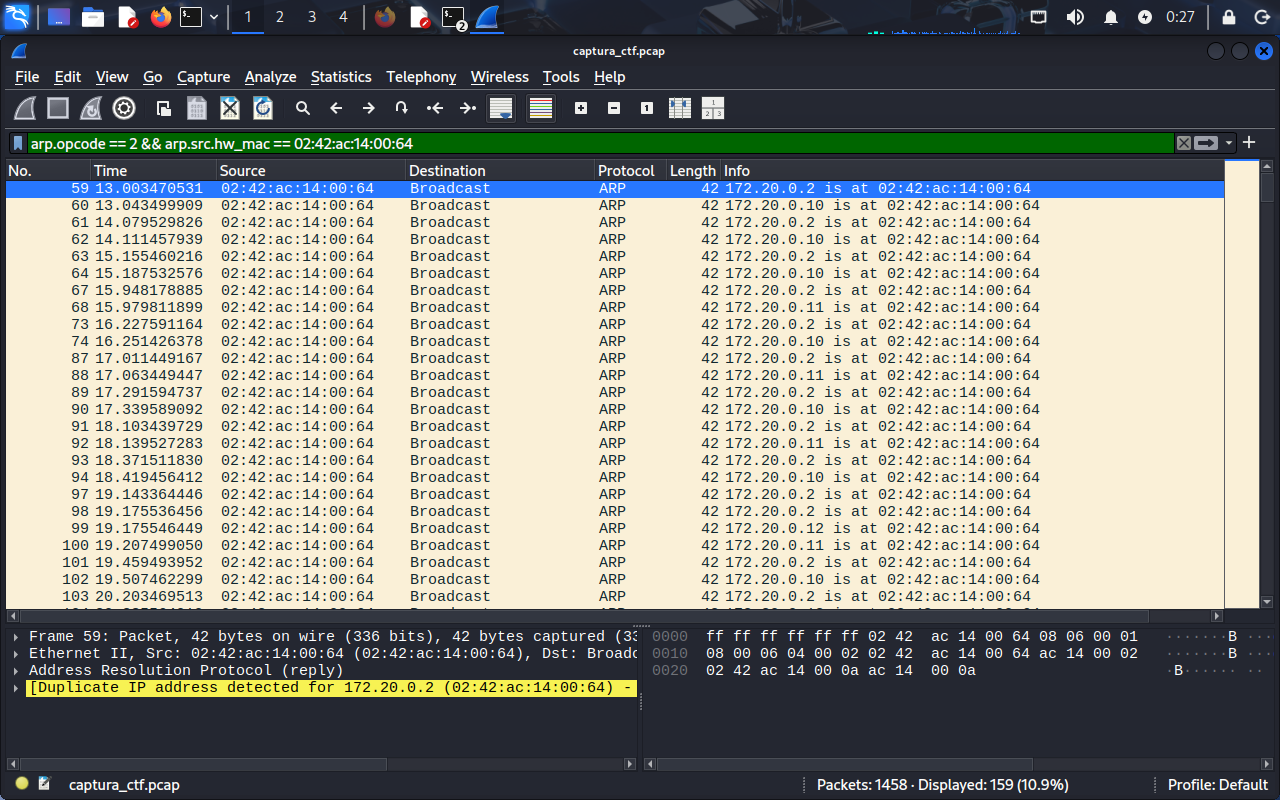
\includegraphics[width=0.85\textwidth]{arpspoofing.png}
\end{center}
\vspace{-0.5em}
\begin{center}
\small Captura de paquetes mostrando ARP Reply falsos del atacante.
\end{center}
\end{frame}

% Slide 16: Wireshark MAC Flooding
\begin{frame}{Evidencia --- Captura MAC Flooding (Wireshark)}
\begin{center}
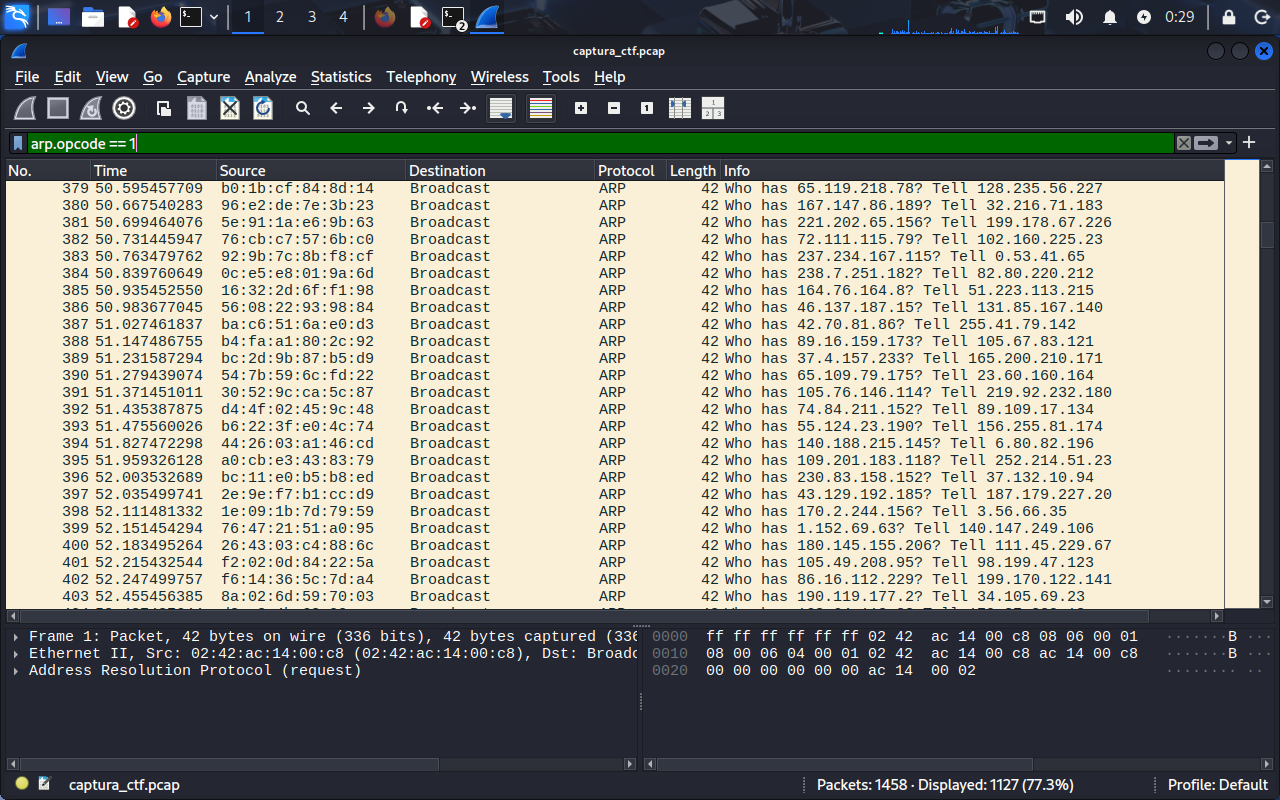
\includegraphics[width=0.85\textwidth]{macflooding.png}
\end{center}
\vspace{-0.5em}
\begin{center}
\small Captura de paquetes mostrando r\'afaga de MACs aleatorias.
\end{center}
\end{frame}

% ============================================================================
\section{Contramedidas}
% ============================================================================

% Slide 17: Contramedidas Recomendadas
\begin{frame}{Contramedidas Recomendadas}
\begin{columns}[T]
\column{0.5\textwidth}
\textbf{Nivel de Switch:}
\begin{itemize}
    \item \textbf{DAI} (Dynamic ARP Inspection)
    \begin{itemize}
        \item Valida paquetes ARP contra tabla DHCP
    \end{itemize}
    \item \textbf{Port Security}
    \begin{itemize}
        \item Limita MACs por puerto
        \item Previene MAC Flooding
    \end{itemize}
    \item \textbf{DHCP Snooping}
    \begin{itemize}
        \item Filtra mensajes DHCP no autorizados
    \end{itemize}
\end{itemize}

\column{0.5\textwidth}
\textbf{Nivel de Red/Aplicaci\'on:}
\begin{itemize}
    \item \textbf{802.1X}
    \begin{itemize}
        \item Autenticaci\'on por puerto
        \item NAC (Network Access Control)
    \end{itemize}
    \item \textbf{TLS/SSL}
    \begin{itemize}
        \item Cifrado extremo a extremo
        \item Mitiga impacto de MitM
    \end{itemize}
    \item \textbf{Monitoreo continuo}
    \begin{itemize}
        \item SIEM + NIDS (Wazuh + Suricata)
        \item Alertas en tiempo real
    \end{itemize}
\end{itemize}
\end{columns}
\end{frame}

% ============================================================================
\section{Conclusiones}
% ============================================================================

% Slide 18: Conclusiones
\begin{frame}{Conclusiones y Lecciones Aprendidas}
\textbf{Conclusiones:}
\begin{itemize}
    \item La Capa 2 es un \textbf{vector de ataque real} frecuentemente ignorado
    \item ARP Spoofing y MAC Flooding son \textbf{f\'aciles de ejecutar} pero dif\'iciles
          de detectar sin herramientas especializadas
    \item La combinaci\'on \textbf{Suricata + Wazuh} proporciona visibilidad efectiva en L2
    \item Docker permite crear \textbf{laboratorios realistas} de forma reproducible
\end{itemize}
\vspace{0.5em}
\textbf{Lecciones aprendidas:}
\begin{itemize}
    \item Suricata requiere t\'ecnicas especiales (\texttt{pkthdr}) para L2
    \item La detecci\'on h\'ibrida (activa + pasiva) es m\'as robusta
    \item CTFd gamifica el aprendizaje de seguridad de forma efectiva
    \item La automatizaci\'on con Docker Compose simplifica despliegues complejos
\end{itemize}
\end{frame}

% ============================================================================
% Slide 19: Preguntas
% ============================================================================
\begin{frame}{}
\begin{center}
\Huge ?`Preguntas?

\vspace{1.5em}
\large \textit{Gracias por su atenci\'on}

\vspace{2em}
\normalsize
Juli\'an Le\'on $\cdot$ James Soto $\cdot$ Mauricio Mantilla\\[0.5em]
\texttt{Redes de Computadoras --- USFQ}\\[0.3em]
Marzo 2026
\end{center}
\end{frame}

\end{document}
